\thispagestyle{empty}
 % 流程图定义基本形状
\tikzstyle{startstop} = [rectangle, rounded corners, minimum width=3cm, minimum height=1cm,text centered, draw=black, fill=red!30]
\tikzstyle{io} = [trapezium, trapezium left angle=70, trapezium right angle=110, minimum width=3cm, minimum height=1cm, text centered, draw=black, fill=blue!30]
\tikzstyle{process} = [rectangle, minimum width=3cm, minimum height=1cm, text centered, draw=black, fill=orange!30]
\tikzstyle{decision} = [diamond, minimum width=3cm, minimum height=1cm, text centered, draw=black, fill=green!30]
\tikzstyle{arrow} = [thick,->,>=stealth]
 
\begin{center}
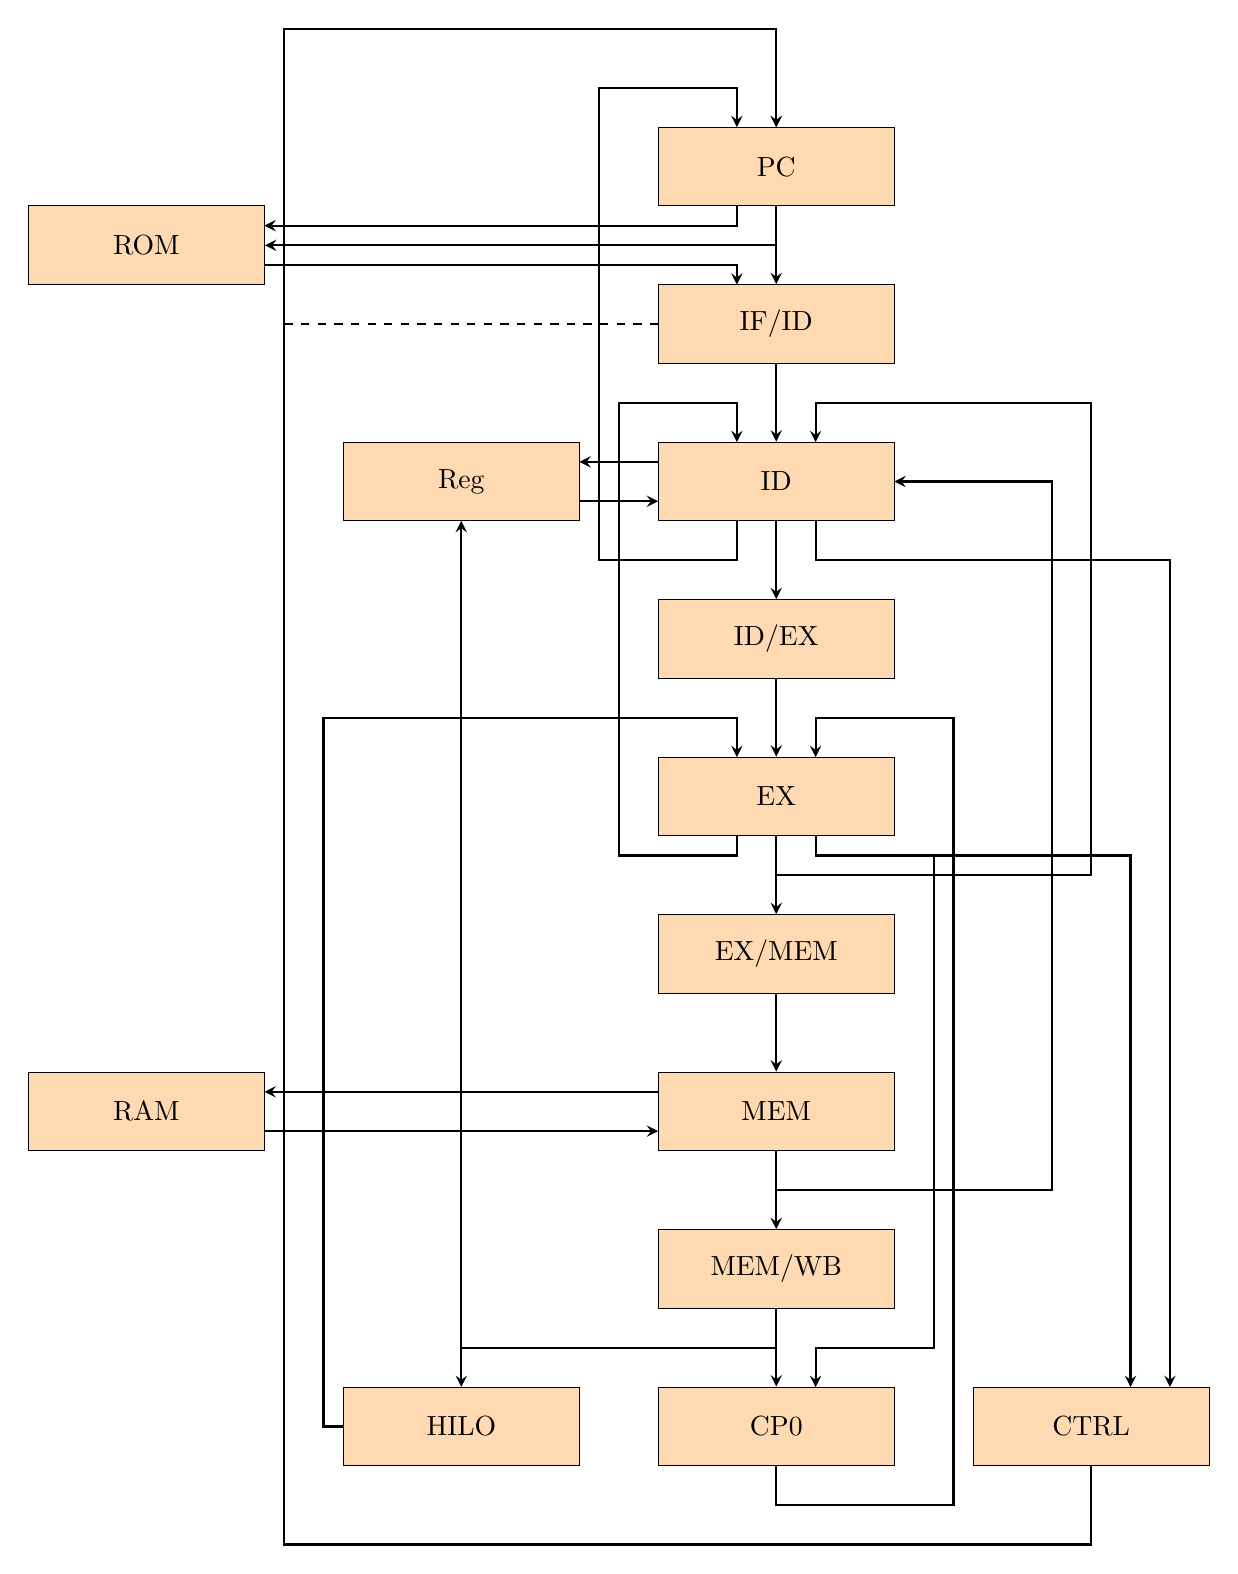
\begin{tikzpicture}[node distance=2cm]
 %定义流程图具体形状
\node (PC) [process] {PC};
\node (IFID) [process, below of=PC] {IF/ID};
\node (ROM) [process, left of=IFID, xshift=-6cm, yshift=1cm] {ROM};
\node (ID) [process, below of=IFID] {ID};
\node (Reg) [process, left of=ID, xshift=-2cm] {Reg};
\node (IDEX) [process, below of=ID] {ID/EX};
\node (EX) [process, below of=IDEX] {EX};
\node (EXMEM) [process, below of=EX] {EX/MEM};
\node (MEM) [process, below of=EXMEM] {MEM};
\node (RAM) [process, left of=MEM, xshift=-6cm] {RAM};
\node (MEMWB) [process, below of=MEM] {MEM/WB};
\node (CP0) [process, below of=MEMWB] {CP0};
\node (HILO) [process, left of=CP0, xshift=-2cm] {HILO};
\node (CTRL) [process, right of=CP0, xshift=2cm] {CTRL};
 
%连接具体形状
%PC
\draw [arrow](PC) -- (IFID);
\draw [arrow](PC) |- (ROM);
\draw [arrow](-0.5, -0.5) -- (-0.5, -0.75) -- (-6.5, -0.75);

%IFID
\draw [arrow](IFID) -- (ID);
\draw [arrow, dashed](-1.5, -2) -| (-6.25, 1.75) -| (0, 0.5);

%ROM
\draw [arrow](-6.5, -1.25) -- (-0.5, -1.25) -- (-0.5, -1.5);

%ID
\draw [arrow](-1.5, -3.75) -- (-2.5, -3.75);
\draw [arrow](ID) -- (IDEX);
\draw [arrow](-0.5, -4.5) |- (-2.25, -5) |- (-0.5, 1) -- (-0.5, 0.5);
\draw [arrow](0.5, -4.5) |- (5, -5) -- (5, -15.5);

%REG
\draw [arrow](-2.5, -4.25) -- (-1.5, -4.25);

%IDEX
\draw [arrow](IDEX) -- (EX);

%EX
\draw [arrow](EX) -- (EXMEM);
\draw [arrow](-0.5, -8.5) |- (-2, -8.75) |- (-0.5, -3) -- (-0.5, -3.5);
\draw [arrow](0, -9) -| (4, -3) -| (0.5, -3.5);
\draw [arrow](0.5, -8.5) |- (4.5, -8.75) -- (4.5, -15.5);
\draw [arrow](2, -8.75) |- (0.5, -15) -- (0.5, -15.5);

%EXMEM
\draw [arrow](EXMEM) -- (MEM);

%MEM
\draw [arrow](MEM) -- (MEMWB);
\draw [arrow](-1.5, -11.75) -- (-6.5, -11.75);
\draw [arrow](0, -13) -| (3.5, -4) -- (1.5, -4);

%RAM
\draw [arrow](-6.5, -12.25) -- (-1.5, -12.25);

%MEMWB
\draw [arrow](MEMWB) -- (CP0);
\draw [arrow](0, -15) -| (-4, -4.5);
\draw [arrow](-4, -15) -- (-4, -15.5);

%CP0
\draw [arrow](0, -16.5) |- (2.25, -17) |- (0.5, -7) -- (0.5, -7.5);

%HILO
\draw [arrow](-5.5, -16) -| (-5.75, -7) -| (-0.5, -7.5);

%CTRL
\draw [arrow](CTRL) |- (-6.25, -17.5) |- (0, 1.75) -- (0, 0.5);

\end{tikzpicture}
\end{center}